\section{Methods}\label{methods}

In this section the underlying concepts and technologies are described. It starts with a brief description of XNAT and OpenStack. For further information about these systems and how they are integrated in the platform see~\cite{wu14}. The section continues with introducing the concept of workflows, the functionalities of WS-PGRADE/gUSE and the DCI-Bridge, which is an important part of gUSE. The last subsection describes a sample application, which has been used throughout the project.

\subsection{XNAT}\label{xnat}

The Extensible Neuroimaging Archive Toolkit (XNAT)~\cite{marcus_extensible_2007} is an opensource archiving software for medical scan data developed by the Neuroinformatics Research Group of the Washingston University in St.Louis.
XNAT provides a graphical user interface to upload and manage scan data.

The main data structures of XNAT are \textit{Projects}, which limit the data access rights of different users.
Each project contains \textit{Subjects} describing the personal data of patients.
Every experiment with a patient is stored as \textit{Session} of the corresponding Subject.

A new Session for ECG data~\ref{applications} can be created in the web interface of XNAT under \textit{New, Experiment, ECG Session}.
The results of data processing algorithms should be stored in the same session as the original experiment data.
In XNAT special data types called \textit{Assessors} exist to store these results.

XNAT also provides a pipeline system, to start data processings from the web interface or automatically whenever a new scan has been uploaded.
The pipeline can execute custom shell scripts and other programs and gives various parameters to the executed program.
These parameters, \textit{Project, Subject, Session, User, Password} and \textit{Host}, are later used by a data processing script to connect to the XNAT API for downloading and uploading scans and results.

In order to perform these actions remotely from the command-line, the corresponding commands used in the workflow implementations~\ref{workflowimplementation} are described in appendix~\ref{xnatapi}.

\subsection{OpenStack}\label{openstack}

OpenStack is a opensource cloud infrastructure software~\cite{openstackhome} provided by the OpenStack Foundation.
With the help of OpenStack an Infrastructure as a Service (IaaS) cloud architecture can be created.
It is used to provide Virtual Machines with limited virtual resources like virtual CPUs, harddrive space and memory.
As user of a VM the underlying physical resources cannot be seen.
Using IaaS it is easy to scale up the virtual resources for higher workloads whenever they are needed.
A Virtual Machine is always booted from an existing harddrive image.
OpenStack can create snapshots, capturing the current state of a VM.
New VMs can also be based on snapshots instead of the original image.

The main infrastructure consists of a Control Node server, a Network Node and several Compute Nodes.
The Control Node can receive various commands, like starting and stopping Virtual Machines, through its Rest APIs (see section~\ref{euca}).
The Network Node manages the public and private IP addresses of the VMs.
In the QMROCT server architecture~\ref{architecture} so called Floating IPs from an IP pool should be assigned to the Virtual Machines to access them within the private network.
The Compute Nodes run the actual Virtual Machines and provide their resources and compute power for this purpose.
In order to scale up the resources new Compute Nodes can be attached to the network.

\subsection{Workflows}\label{workflows}

Applications consist of executable programs.
They usually take input in the form of command-line parameters or files and produce output files.
Some programs depend on the output of other programs, so that a mechanism is needed to ensure that all required inputs have been produced successfully before the program runs.
The workflow itself is a description or recipe how to link the executables together and are often stored in xml formats.

In terms of a workflow, every program is described as job, which can consist of one executable file or, as in gUSE, can be a .zip file containing a set of executable files.
Every job has input and output ports, where each port has a number to identify it.
There can only be one file assigned to each port, which is then used to execute the program.
Every output port of one job can be linked to an input port of another program.
A system like gUSE, which implements workflows, ensures that the all necessary inputs are available before the job is started.
The produced data is then transported to the expected location where the next job can use it.
When a job fails, it can resume this single job after the problem has been fixed.
There is no need to process all the successfully finished jobs again.
One of the most important feature of the ports is the support of naming conventions.
An input file assigned to a port is renamed, so that the program can find it in the storage.
The program also produces files that are named in a special way.
This name must be specified for the output port, so that the workflow system can keep track of the produced files.
Different jobs that have linked outputs and inputs can follow different naming conventions.

The input files can be given to input ports one by one or by using parameters sweeps.
Parameter sweeps include several input files in one .zip file, so that they are uploaded at once and are then processed in a row.
When there are several input ports, the inputs of the different ports can be combined linearly by matching the first input of the first port with the first input of the second port and the second input of the first port with the second input of the second port.
Another method combines the inputs like a cross product, so that also the first input of the first port is combined with the second input of the second port and vice versa.

\subsection{WS-PGRADE/gUSE}\label{guse}

Grid and cloud User Support Environment (gUSE) is an opensource workflow management system developed at the Laboratory of Parallel and Distributed Systems in Hungaria.
WS-PGRADE is a collection of several gUSE Java Enterprise services that are combined to form a full featured e-science portal.
It provides a user-interface based on the opensource portal software Liferay.

The web portal is used to create and manage workflows. In order to create a new workflow three steps are necessary. First a graph is created using a Java Applet named graph editor, which is provided on the portal. With the graph editor new jobs can be created and their ports can be connected (see section~\ref{workflows}). Figure~\ref{fig:grapheditor} shows a graph in the editor. The jobs are symbolized by yellow squares. Input ports are green, while output ports are gray. The arrows symbolize connections.
The graph is used to create a concrete workflow instance, which in the last step has to be configured.
The concrete workflows are shown in the user interface as can be seen in figure~\ref{fig:interfaceworkflows}.
During the configuration the executable programs and necessary command-line parameters are assigned to each job and input files are uploaded and assigned to the ports.
Also previously configured middlewares can be selected, which define the platform to execute the workflows (see section~\ref{dci}).
The finalized workflow is then submitted to be executed.
The details button shows the status of the submitted workflows, wether they are running, finished or failed with an error.
Once a workflow is finished the resulting files, defined by the output ports, can be downloaded as a .zip file.
Failed workflows can be resumed after the problem has been solved.

\begin{figure*}%[!b]
                \centering
                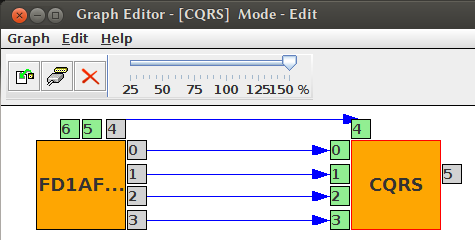
\includegraphics[width=1.0\columnwidth]{images/graph-editor.png}
                \caption{Graph editor of WS-PGRADE}
                \label{fig:grapheditor}
\end{figure*}

\begin{figure*}%[!b]
                \centering
                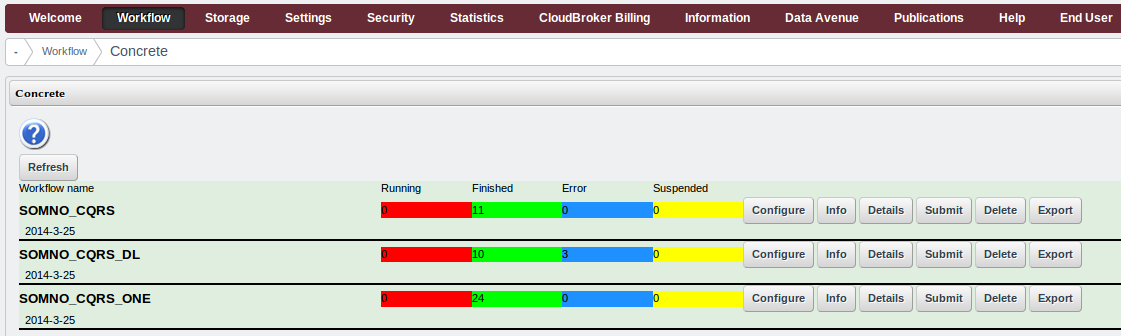
\includegraphics[width=2.0\columnwidth]{images/interface-workflows.png}
                \caption{List of concrete workflows in the web portal}
                \label{fig:interfaceworkflows}
\end{figure*}

In order to control workflows automatically gUSE provides two different APIs.
The Application-Specific Module API (ASM) provides access to gUSE functionality for Java developers.
For remote server calls a Rest API is provided. It can be used for basic workflow controls like starting, stopping, resuming and gathering status information.
The latter is more suitable for the loose coupling of the given QM-ROCT server infrastructure (see section~\ref{architecture}), because the functionality to call the API can be implemented on another server and not inside the gUse Java environment.

\subsection{DCI-Bridge}\label{dci}

The DCI-Bridge is part of gUSE and connects the workflow system with different types of Distributed Computing Infrastructures (DCI).
These middlewares are for example grid or cloud infrastructures, where applications can be executed.
The DCI-Bridge is a generic interface receiving requests from the workflow system.
Different DCI plugins handle these request for different infrastructure types.
To connect to a cloud infrastructure the DCI-Bridge provides a CloudBroker and a EC2 plugin.
CloudBroker is an external service which is used to connect to a cloud.
Because the SOMNO.Netz server architecture is encapsulated in a private network, which can not be reached from outside, this is not a suitable option.
Instead the EC2 plugin can be used, which connects to the cloud directly via the EC2 interface of OpenStack (see section~\ref{openstack}), using the opensource command-line software euca-tools (see section~\ref{euca}).
The plugin is able to orchestrate the cloud resources, like starting and stopping VMs whenever they are needed.
It will start a new VM when a workflow is submitted and process the data in the cloud.
The VM is not being shut down immediately after it has been used.
The system waits for more submits to reuse the same VM instance.
Only if it has not been used for a certain time it is being terminated again.
In the web interface the number of VM instances running at a time can be limited, to control the load of the cloud. 
An image or snapshot, which is used to create the Virtual Machine, is also specified in the DCI settings.
The Virtual Machine image itself must have a Slave DCI-Bridge tool installed.
This tool runs a web server and receives the jobs with the data and executables from the server side DCI-Bridge.
It executes the jobs and sends the results back to gUSE.
A VM image with a properly configured Slave DCI-Bridge can be downloaded~\cite{slavedci}.

\subsection{Nova Client \& Euca Tools}\label{euca}
Nova Client~\cite{nova} is a command line tool provided by OpenStack, to send control requests to an OpenStack control server. It communicates with the OpenStack standard remote API.

Euca2ools~\cite{eucatools} is a python library and a set of command line tools provided by Eucalyptus Systems, to control a remote EC2 API of a cloud middleware like Amazon Elastic Compute Cloud (Amazon EC2)~\cite{amazon}.
OpenStack also provides an EC2 API besides the Nova API.
Euca2ools is used by the gUSE DCI-Bridge to create and terminate VM instances and therefore must be installed on the gUSE server.

\subsection{Sample Applications}\label{applications}

The application CQRS~\cite{krefting10} processes polysomnographic electrocardiogram (PSG-ECG) data and is used as sample for modeling workflows throughout this project.
The application consists of two Matlab algorithms, which are are executed using a shell script.
To run the algorithms a Matlab Compiler Runtime (MCR) must be installed.
The path of the MCR is given to the shell scripts as command-line parameter.
Matlab files are not executed directly, but with a run script located in the same directory.
The first algorithms takes an ECG data file (ecg.dat) and a header file (ecg.hea) as input and produces three different files (ecg\_fd1.dat, ecg\_af2.dat, ecg\_df2.dat) as output.
All five files are given to the second algorithm as input parameters, which produces the final output file (ecg\_cqrs.dat).
The original input files can be stored in XNAT (see section~\ref{xnat}) as scan files in a session.
The output files are stored as assessment data in the same session as the scan files.

\subsection{Workflow Repositories}\label{repositories}

Workflow repositories store given workflows and their settings including the application executables.
gUSE provides a local repository, which can be reached from the portal user interface.
It also supports exporting the workflow with the application binaries, input data and an XML description of the contained jobs and ports.

In order to publish workflows a remote repository \cite{somnocqrs} provided by the SHIWA project can be used.
gUSE provides a build-in upload functionality to connect to remote repositories.